%Dies ist die Hauptseite des Dokumentes. Es werden u. a. alle Kapitel,
%Einstellung im Header eingebunden.
%Veränderungen müssen in folgenden Dateien vorgenommen werden:
      %- Layout.tex
      %- newComments.tex
      %- Titelseite
      %- Versionsübersicht
      %- einzelne Kapitel (evtl. erweitern)


% Definition von globalen Parametern, die derzeit auf der Titelseite und in der
% Kopfzeile verwendet werden. Der in <> gesetzte Text ist zu verändern.

\newcommand{\praktikumTitel}{WiReLib}
\newcommand{\projektTitel}{WiReLib}


%Hier sind alle Einstellungen enthalten, die sich auf das Seiten- und
%Dokumentenlayout beziehen

\documentclass[
  11pt,                % Schriftgröße
  DIV12,
  german,              % für Umlaute, Silbentrennung etc.
  oneside,            % einseitiges Dokument
  titlepage,          % es wird eine Titelseite verwendet
  parskip=half,        % Abstand zwischen Absätzen (halbe Zeile)
  headings=normal,      % Größe der Überschriften verkleinern
  captions=tableheading,  % Beschriftung von Tabellen unterhalb ausgeben
  final                % Status des Dokuments (final/draft)
]{scrreprt}            %


%------Ändern von Schriftschnitten - (Muss ganz am Anfang stehen !) ------------
\usepackage{fix-cm}

%------Umlaute -----------------------------------------------------------------
%   Umlaute/Sonderzeichen wie äüöß können direkt im Quelltext verwenden werden.
%    Erlaubt automatische Trennung von Worten mit Umlauten.
\usepackage[T1]{fontenc}
\usepackage[utf8]{inputenc}

%------Anpassung der Landessprache----------------------------------------------
\usepackage{ngerman}

%------Einfache Definition der Zeilenabstände und Seitenränder------------------
\usepackage{geometry}
\usepackage{setspace}
\usepackage{xspace}

%------Schriftgrößenanpassung von einzelnen Textpassagen------------------------
\usepackage{relsize}

%------Trennlinien in Kopf- und Fusszeile
\usepackage[headsepline, footsepline, ilines]{scrpage2}

%------Grafiken-----------------------------------------------------------------
\usepackage{graphicx}

%------Packet zum Sperren, Unterstreichen und Hervorheben von Texten------------
\usepackage{soul}

%------ergänzende Schriftart----------------------------------------------------
\usepackage{helvet}

%------Lange Tabellen-----------------------------------------------------------
\usepackage{longtable}
\usepackage{array}
\usepackage{ragged2e}
\usepackage{lscape}

%------PDF-Optionen-------------------------------------------------------------
\usepackage[
  bookmarks,
  bookmarksopen=true,
  colorlinks=true,
  linkcolor=black,        % einfache interne Verknüpfungen
  anchorcolor=black,      % Ankertext
  citecolor=black,        % Verweise auf Literaturverzeichniseinträge im Text
  filecolor=black,        % Verknüpfungen, die lokale Dateien öffnen
  menucolor=black,        % Acrobat-Menüpunkte
  urlcolor=black,         % Farbe für URL-Links
  backref,                % Zurücktext nach jedem Bibliografie-Eintrag als
                          % Liste von Überschriftsnummern
  pagebackref,            % Zurücktext nach jedem Bibliografie-Eintrag als
                          % Liste von Seitenzahlen
  plainpages=false,       % zur korrekten Erstellung der Bookmarks
  pdfpagelabels,          % zur korrekten Erstellung der Bookmarks
  hypertexnames=false,    % zur korrekten Erstellung der Bookmarks
  linktocpage             % Seitenzahlen anstatt Text im Inhaltsverzeichnis
                          % verlinken
  ]{hyperref}

%-----Glossar-Optionen----------------------------------------------------------
\usepackage{translator}
\usepackage[				   %
acronym,		% ein Abkürzungsverzeichnis erzeugen
toc,			% Taucht im Inhaltsverzeichnis auf
]				   
{glossaries}
\makeglossaries

\usepackage{xcolor}
\definecolor{lightergray}{rgb}{0.9,0.9,0.9}

\usepackage{listings}
\lstset{numbers=left, numberstyle=\tiny, numbersep=5pt,
breaklines=true, backgroundcolor=\color{lightergray},
basicstyle=\ttfamily,
}
\usepackage{booktabs}
      % enthält eingebundene Packete

%------Seitenränder-------------------------------------------------------------
\geometry{verbose,                     % zeigt die eingestellten Parameter beim
                                       % Latexlauf an
      paper=a4paper,                   % Papierformat
      top=25mm,                        % Rand oben
      left=25mm,                       % Rand links
      right=25mm,                      % Rand rechts
      bottom=45mm,                     % Rand unten
      pdftex                           % schreibt das Papierformat in die
                                       % Ausgabe damit Ausgabeprogramm
                                       % Papiergröße erkennt
  }

%Seitenlayout
\onehalfspace        % 1,5-facher Abstand

%------Kopf- und Fußzeilen -----------------------------------------------------
\pagestyle{scrheadings}

%------Kopf- und Fußzeile auch auf Kapitelanfangsseiten ------------------------
\renewcommand*{\chapterpagestyle}{scrheadings}

%------Schriftform der Kopfzeile -----------------------------------------------
\renewcommand{\headfont}{\normalfont}

%------Kopfzeile----------------------------------------------------------------
\setlength{\headheight}{21mm}        % Höhe der Kopfzeile
\ihead{\large{\textsc{\praktikumTitel}}\\    % Text in der linken Box
       \small{\projektTitel}}
\chead{}                            % Text in der mittleren Box

%----Fusszeile
\cfoot{}                            % Text in mittlerer Box
\ofoot{\pagemark}                    % Seitenzahl in rechter Box
          % Diese Datei enthält alle
                                          % Layouteinstellungen

% Kapitel 9
%-------------------------------------------------------------------------------
%Hier werden Fachbegriffe und Abkürzungen erklährt.
% Verwendet werden diese Begriffe mit \gls{name} oder \Gls{name} wenn der Anfang
% groß geschrieben sein muss.
%
%%	Beispiel unter: http://ewus.de/tipp-1029.html
%%	und natürlich Erkärung mit dem Befehl
%texdoc glossaries

\newacronym{UB}{UB}{Universitätsbibliothek}
\newacronym{GITZ}{GITZ}{Gauß-IT-Zentrum}
\newacronym{LDAP}{LDAP}{Lightweight Directory Access Protocol\protect\glsadd{glos:LDAP}}

% nur über \gls{LDAP} verwenden.
\newglossaryentry{glos:LDAP}{name=Lightweight Directory Access Protocol,
description={LDAP ist ein Verzeichnisdienst der von der TU Braunschweig für die Benutzerauthentifizierung bereit gestellt wird}
}
\newglossaryentry{glos:https}{name=Hypertext Transfer Protocol Secure,
description={Hypertext Transfer Protocol Secure ist die verschlüsselte Variante
vom Hypertext Transfer Protocol und ist eine zertifiktasbasierende sichere
Übertragungstechnik}
}
\newglossaryentry{glos:sqlite}{name=SQLite,
description={SQLite ist eine Relationale Datenbank die von Python direkt zur Verfügung gestellt wird}
}
\newglossaryentry{glos:copdes}{name=Corporate Design,
description={Das Corporate Design ist das gemeinsame Erscheinungsbild eine Unternehmens. Dies bezieht sich unter anderem auf Kommmunikationsmittel, Werbemittel und Internetauftritte}
}
\newglossaryentry{glos:unicode}{name=Unicode,
description={Der Unicode ist ein Standard, in dem jedes sinntragende Schirftzeichen einem digitalen Code zugeordnet werden soll. Dadurch sollen Kompatibilitätsproblem aufgrund verschiedener Kodierungen in verschiedenen Ländern umgangen werden}
}
\newglossaryentry{glos:thmefi}{name=Thunderbird Message Filter,
description={Der Thunderbird Message Filter ist eine einfache Möglichkeit E-Mails in dem Programm Mozilla Thunderbird zu durchsuchen}
}
\newglossaryentry{glos:BibTeX}{name=Bib\TeX,
description={Bib\TeX\xspace ist ursprünglich eine Erweiterung für \LaTeX\xspace zur Verwaltung eines Literaturverzeichnisses für wissenschaftliche Publikationen. Inzwischen ist das Format auch unter anderen Textverarbeitungsprogrammen benutzbar}
}
\newglossaryentry{glos:Allegro}{name=Allegro,
description={Allegro ist das Datenbanksystem, welches in der Universitätsbibliothek der TU Braunschweig entwickelt und verwendet wird}
}
\newglossaryentry{glos:regex}{name=Reguläre Ausdrücke,
description={Reguläre Ausdrücke sind ein Mittel der Theoretischen Informatik um Sprachen (dt. Wortmengen) zu beschreiben. In der angewanten Informatik werden diese Ausdrücke noch heute oft verwendet. Mit Regulären Ausdrücken ist eine präzise Beschreibung eines Suchwortes möglich}
}
\newglossaryentry{glos:ext}{name=Externe,
description={Der Begriff \emph{Externe} beschreibt alle Personen die nicht am System angemeldet sind, also \mbox{z.\,B.}\xspace Mitarbeiter anderer Institute mit einem Ausleihwunsch}
}



\newcommand{\BibTeX}{\gls{glos:BibTeX}\xspace}
\newcommand{\zB}{\mbox{z.\,B.}\xspace}
%------Beginn des Gesamtdokumentes----------------------------------------------
\begin{document}

%------Eingebundene Seiten, Verzeichnisse bzw. Kapitel--------------------------
% Dies ist die Titelseite des Grobentwurfs.
% Die in "<...>" sind zu ersetzen
% Die Ausgabe darf 1 Seite nicht überschreiten, also ggf. Abstände anpassen
% Die Angabe in [...] gibt den Abstand nach der entsprechenden Zeile an.


%----Stil dieser Seite----------------------------------------------------------
\thispagestyle{plain}      % Kopfzeile bleibt leer

%----Beginn der Titelseite------------------------------------------------------
\begin{titlepage}

%----zentrierte Ausrichtung über die gesamte Seite----------------------------
\begin{center}

%----Titel des Praktikum (\praktikumTitel in newComments zu verändern)--------
{\relsize{4}{\textbf{\textsc{\praktikumTitel}}}}\\[3ex]%[5ex]

%----Titel des Teilprojektes (\projektTitel in newComments verändern)---------
{\relsize{3}{\textbf{\textsc{\projektTitel}}}}\\[3ex]%[5ex]

Software-Entwicklungspraktikum (SEP)\\
Sommersemester 2012\\[4ex]%[6ex]

{\relsize{3}\so{\textbf{Grobentwurf}}}\\[4ex]%[5ex]

%----eingebundenes Logo der TU--------------------------------------------------

\includegraphics[scale=0.8]{bilder/carolo.jpg}\\[4ex]%[5ex]

%----Daten des Auftraggebers
Auftraggeber\\
Technische Universität Braunschweig\\
Wissenschaftliches Rechnen\\
Prof. Hermann G. Matthies\\
Hans-Sommer-Straße 65\\
D-38092 Braunschweig\\[1ex]%[2ex]
Betreuer: Elmar Zander\\[4ex]%[5ex]

% ----Tabelle der Praktikumsteilnehmer------------------------------------------
Auftragnehmer:
\begin{tabular}{l<{\hspace{20mm}} l<{\hspace{30mm}}}\\
  Name                   &   E-Mail-Adresse\\      % Zeilenüberschift
  \hline                    % Linie unterhalb der Zeilenüberschrift
  %----Nachfolgend alle Namen und E-Mail-Adressen der Teilnehmer einfügen
  Eric Anders 		& eric.anders89@web.de\\
  Johann Hong 		& johann.hong@googlemail.com\\
  Jörn Hameyer 		& j.hameyer@tu-bs.de\\
  Marco Melzer 		& marco.melzer@tu-braunschweig.de\\
  Markus Dietrich 	& markus.dietrich@tu-bs.de\\
  Philipp Offensand & PhilippOffensand@gmx.de\\
  Stephan Sobol 	& stephan.sobol@web.de\\
  Theodor van Nahl 	& t.nahl@tu-bs.de
\end{tabular}\\[1ex]%[2ex]

Braunschweig, 24.04.2012

\end{center}
\end{titlepage}

                      % Titelseite
%Diese Datei dient der Versionskontrolle. Sie ist vollständig zu bearbeiten.

%----Überschrift------------------------------------------------------------
{\relsize{2}\textbf{Versionsübersicht}}\\[2ex]

%----Start der Tabelle------------------------------------------------------
\begin{longtable}{|m{1.78cm}|m{1.59cm}|m{2.86cm}|m{1.9cm}|m{5.25cm}|}

  \hline                                              % Linie oberhalb

  %----Spaltenüberschriften------------------------------------------------
  \textbf{Version}  &    \textbf{Datum}  &    \textbf{Autor}  &
  \textbf{Status}   &    \textbf{Kommentar}       \\  %Spaltenüberschrift
  \hline                                              % Gitterlinie

  %----die nachfolgeden beiden Zeilen so oft wiederholen und die ... mit den
  %    entsprechenden Daten zu füllen wie erforderlich
  0.1   &    16.05.2012    &    Theodor van-Nahl    &   in Bearbeitung     &    Analyse der Produktfunktionen F100-F200\\       % Eintrag in Zeile
  \hline                                              % Gitterlinie unten
  0.2   &    17.05.2012    &    Jörn Hameyer    &   in Bearbeitung     &    Analyse der Produktfunktionen F226-F229\\       % Eintrag in Zeile
  \hline
  0.3   &    18.05.2012    &    Stephan Sobol    &   in Bearbeitung     &    Analyse der Produktfunktionen F220-F225\\       % Eintrag in Zeile
  \hline
  0.4   &    18.05.2012    &    Philipp \mbox{Offensand}    &   in Bearbeitung     &    Qualitätsanalyse\\       % Eintrag in Zeile
  \hline
  0.5   &    18.05.2012    &    Markus Dietrich    &   in Bearbeitung     &    Analyse der Produktfunktionen F230-F302\\       % Eintrag in Zeile
  \hline
  0.6   &    18.05.2012    &    Johann Hong    &   in Bearbeitung     &    Analyse der Produktfunktionen F210-F214\\       % Eintrag in Zeile
  \hline
  0.7   &    18.05.2012    &    Marco Melzer    &   in Bearbeitung     &    Einleitung\\       % Eintrag in Zeile
  \hline
  0.8   &    18.05.2012    &    Philipp \mbox{Offensand}    &   in Bearbeitung     &    Komponentenspezifikation\\       % Eintrag in Zeile
  \hline
  0.9   &    19.05.2012    &    Theodor van-Nahl    &   in Bearbeitung     &    Analyse der Produktfunktion F201-F210\\       % Eintrag in Zeile
  \hline
  0.10   &   21.05.2012    &    Marco Melzer    &   in Bearbeitung     &    Schnittstellenspezifikation\\       % Eintrag in Zeile
  \hline
  0.11   &   22.05.2012    &    Joahann Hong    &   in Bearbeitung     &    Verteilungsentwurf\\       % Eintrag in Zeile
  \hline
  0.12   &   23.05.2012    &    Jörn Hameyer,\newline Stephan Sobol    &   in Bearbeitung     &    Protokolle für die Benutzung der Komponenten\\       % Eintrag in Zeile
  \hline
  1.0   &    23.05.2012    &    sämtliche Auftragnehmer    &   abgenommen     &    \\       % Eintrag in Zeile
  \hline
  

%----Ende der Tabelle------------------------------------------------------
\end{longtable}

Status: "`in Bearbeitung"' oder "`abgenommen"'
Kommentar: hier eintragen, was ge\"andert bzw. ergänzt wurde


Hinweis zum Template:
Dieses Template enth\"ult Hinweise, die alle kursiv geschrieben sind. Alles
Kursivgeschriebene ist selbstverst\"andlich bei Abgabe zu entfernen sind.
Angaben in <\ldots> sind mit dem entsprechendem Text zu f\"ullen.  \"Uberz\"ahlige
Kapitel, d.h. Kapitel, die nicht bearbeitet werden m\"ussen, da sie nicht der
Aufgabenstellung entsprechen, bitte entfernen.

Aufgabe des Grobentwurfs: Aufgabe dieses Dokumentes ist es, die Architektur des
Systems zu beschreiben und die daraus resultierenden Pakete durch die
Definition von Schnittstellen zu Komponenten auszubauen.
       % Versionsübersicht

\tableofcontents                          % Inhaltsverzeichnis wird automatisch
                                          % generiert
\listoffigures                            % ebenso das Abbildungsverzeichnis

%----Kapitel des Feinentwurfs, die mit Inhalt zu füllen sind--------------------
% Kapitel 1
% Die Unterkapitel können auch in separaten Dateien stehen,
% die dann mit dem \include-Befehl eingebunden werden.
%-------------------------------------------------------------------------------

\chapter{Einleitung}
Die Datenbank WiReLib repräsentiert die den Bestand der Bibliothek für das Institut für Wissenschaftliches Rechnen.
Auf diese Datenbank können Nutzer über ein Web-Interface zugreifen um Dokumente zu suchen und sich nach der Anmeldung Dokumente auszuleihen.

\section{Projektdetails}
Die Funktionalitäten gliedern sich in drei Teilbereiche.
Diese Bereiche bündeln die Anforderungen, die im Pflichtenheft spezialisiert
worden sind.

\begin{figure}[h]
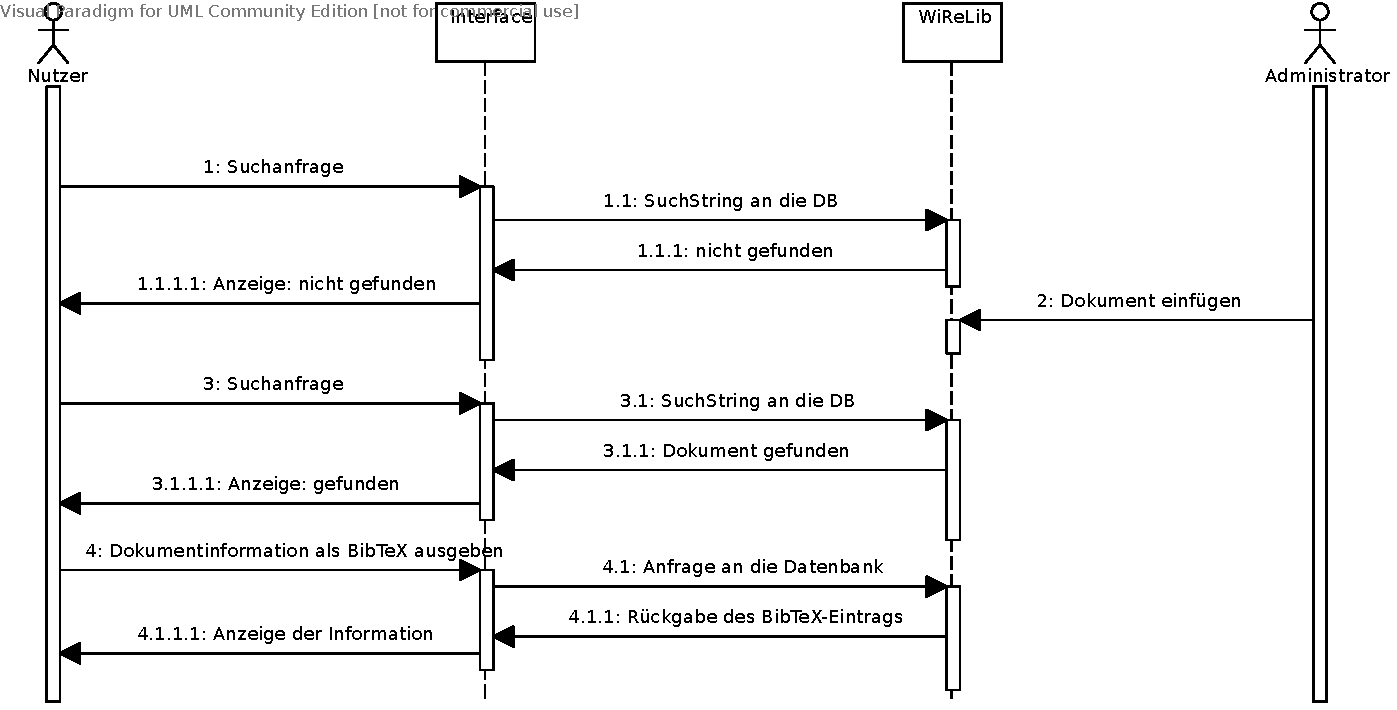
\includegraphics[width=0.8\linewidth]{bilder/Seq-Uebersicht.pdf}
\caption[Übersichtssequenzdiagramm]{Übersichtssequenzdiagramm}
\label{fig:Seqü}
\end{figure}

\subsection{Client}
Über das Web-Interface erhält der als Client fungierende Browser Zugriff auf die Datenbank und kann verschiedene Funktionen nutzen.

\subsection{Server}
Auf dem Server läuft die Anwendung, welche verschiedene Funktionen zum Auslesen und Verwalten der Datenbank bereitstellt. 
Auch stellt der Server die Datenbank bereit und baut eine sichere Verbindung zum Client auf.

\subsection{Datenbank}
In der Datenbank werden die Dokumenente sowie die Nutzerrechte verwaltet.
Auch werden Daten zu den einzelnen Nutzern gespeichert um diese zu identifizieren und im Falle des Ablaufs der Verleihfrist zu benachrichtigen.
               % Kapitel 1
% Kapitel 2 mit den entsprechenden Unterkapiteln
% Die Unterkapitel k\"onnen auch in separaten Dateien stehen,
% die dann mit dem \include-Befehl eingebunden werden.
%----------------------------------------------------------------------------

\chapter{Testplan}
%Der Testplan ist das zentrale Dokument der Qualit\"atssicherung und wird daher
%fr\"uhzeitig erstellt. Hier wird Umfang und Vorgehensweise der Qualit\"atssicherung
%beschrieben. Außerdem werden Testgegenst\"ande und deren zu testenden
%Eigenschaften bzw. Funktionen identifiziert. Ferner werden die
%durchzuf\"uhrenden Maßnahmen und die daf\"ur verantwortlichen Personen definiert.
%Falls erforderlich sollte hier auch auf allgemeine Risiken eingegangen werden.

\section{Zu testende Komponenten}

%Hier sind s\"amtliche zu testenden Objekte einschließlich der Versionsnummer aufzuf\"uhren.
%Ebenso ist anzugeben, auf welchem Medium die Software vorliegt, ob dies einen Einfluss auf Hardwareanforderungen hat
%und ob die Software vor Testbeginn in irgendeiner Weise transformiert werden muss. Außerdem wird auf zum
%Objekt geh\"orende Dokumentation der Komponente (Lasten-, Pflichtenheft, Grob-
%bzw. Feinentwurf) referenziert.

Es müssen die Komponenten Views, Templates und Models getestet werden.
Dabei werden die Komponenten Templates und Models durch die Funktionen der
Komponenten Views und Admin gestestet. Da es sich um eine Webanwendung handelt
ist zu beachten, dass unterschiedliche Clienten (Browser) benutzt werden.

Die Software kann online in der Repository, lokal auf der Festplatte oder einem
anderem Speichermedium vorliegen. Es ist allerdings sicherzustellen, dass die
Software korrekt auf dem Server konfiguriert wird (s. Feinentwurf Kapitel 5)
sowie eine funktionierende (Internet-) Verbindung zwischen Server und Client
besteht.

\section{Zu testende Funktionen}
%Dieser Punkt beinhaltet alle Eigenschaften bzw. Funktionen und deren
%Kombinationen, die zu testen sind.

%S\"amtliche Funktionalit\"aten, die getestet werden sollen, werden hier aufgef\"uhrt.
%Dabei sind auf die vorangegangenen Dokumentationen zu referenzieren
%(Pflichtenheft, Grob- und Fein-entwurf) und die dortigen Funktions-IDs zu
%verwenden!\\ Beispiel: /F100/ : Benutzer Login

\begin{itemize}
\item /F103/: Mailtexte ändern
\item /F200/: \BibTex - Import %Theo
\item /F201/: Webinterface - Import
\item /F202/: Editieren von Dokumenten
\item /F212/: Erweiterte Suche %Markus
\item /F213/: Suche mit regulären Ausdrücken %Markus
\item /F214/: Sortierung der Suche %Eric
\item /F221/: Ausleihe an Externe %Marco
\item /F222/: Ausleihe übertragen %Marco
\item /F223/: Ausleihe zurückgeben
\item /F224/: Ausleihe vermisst melden
\item /F225/: Ausleihe verloren melden
\item /F226/: Ausleihfrist abgelaufen
\item /F227/: Ausleihhistory
\item /F228/: Derzeitiger Leihender %Markus
\item /F229/: Entleihliste %Johann 
\item /F230/: \BibTex - Export %Theo
\item /F231/: Universitätsbibliotheks - Export
\end{itemize}

\section{Nicht zu testende Funktionen}

%(optional; auszuf\"ullen, falls es Funktionen gibt, die nicht getestet werden
%sollen)\\

%Hier werden alle Eigenschaften bzw. Funktionen und Funktionskombinationen
%aufgelistet, die nicht getestet werden.
%\textbf{ Es sollte begr\"undet werden, warum diese nicht getestet werden.} Es
%versteht sich von selber, dass alle Muss-Funktionalit\"aten des Pflichtenheftes
%(Abschnitt 1.1) getestet werden m\"ussen.

Die folgenden Funktionen werden nicht getestet, da sie aus
Django-Built-In-Funktionen bestehen. Diese Funktionen wurden bereits bei der
Entwicklung von Django ausführlich und professionell getestet.

\begin{itemize}
\item /F100/: Anmeldung
\item /F203/: Löschen von Dokumenten
\item /F210/: Generelle Suche
\item /F211/: Suche mit erweiterten Ausdrücken
\item /F220/: Ausleihe
\item /F300/: Benutzerverwaltung
\item /F301/: Rechtezuweisung für Rollen
\item /F302/: Benutzer Rolle(n) zuweisen
\end{itemize}

\section{Vorgehen}
%Die allgemeinen Vorgehensweisen f\"ur die einzelnen zu testenden Funktionen und
%Funktionskombinationen werden hier beschrieben. Die Beschreibung sollte
%detailliert genug sein, um die Hauptaktivit\"aten und deren Zeitbedarf absch\"atzen
%zu k\"onnen.

%Es ist zu beachten, dass f\"ur alle wichtigen Funktionalit\"aten das Verfahren
%angegeben wird. Dies gew\"ahrleistet, dass diese Funktionalit\"aten ad\"aquat
%getestet werden.

%Es ist zu dokumentieren, welche Aktivit\"aten, Techniken und Werkzeuge ben\"otigt
%werden, damit die Funktionalit\"aten getestet werden k\"onnen.

%Beispiel f\"ur Vorgehen (unvollst\"andige Liste):\\
%a) Komponenten- und Integrationstests\\
%Klassen werden mit JUnit-Testf\"allen gepr\"uft. Vor Beginn der Implementierung
%werden bereits Blackbox-Testf\"alle erstellt, die dann begleitend zur
%Implementierung genutzt werden ("`Test first"'). Nach Abschluss der
%Implementierung einer Komponente wird diese dann durch Whitebox-Tests
%gepr\"uft.\\
%Der Integrationstest der Klassen und Komponenten erfolgt nach dem
%Bottom-Up-Prinzip. Anfangs muss die Integration der Datenbankanbindung und den
%entsprechenden Data-Access-Objects (DAO) gepr\"uft werden, da das Mapping der
%Datenbank auf Objekte die unterste Schicht des Projektes bildet. Dieser
%Testabschnitt wird durch die Schnittstellentests abgedeckt.
%Die Komponenten werden damit unter Ber\"ucksichtigung ihrer Abh\"angigkeiten
%konkret in folgender Reihenfolge integriert: \ldots\\
%(Hier kommt das konkrete Vorgehen bei der Integration: Welche Klassen werden
%zusammen getestet, welche kommen dann dazu etc. Das kann man z.B. auch sch\"on in
%Form eines Baumes aufzeigen.)
%b) Funktionstests\\
%Die Anwendungsf\"alle aus der Anforderungsspezifikation werden \"uber das
%Web-Interface gepr\"uft. Mindestanforderung hierf\"ur ist es, jeden Fall einmal auf
%seine korrekte Funktionalit\"at zu testen.\\
%c) \ldots

Aufgrund der Struktur des Projektes werden sämtliche Tests als Funktionstests
über das Webinterface getestet. Dabei werden Firefox, Opera, Chrome, IE 9 als
Browser benutzt um zu gewährleisten, dass das Webinterface auf möglichst vielen
Clientsystemen funktioniert. Als weiteres Werkzeug verwenden wir das Django
testing Environment

\section{Testumgebung}
%Die genutzte Testumgebung(en) bitte hier angeben und kurz beschreiben.\\
%Beispiel: JUnit Testsuite, lokal installierter Web Application Server, \ldots

Als Testumgebung auf dem Server wird der lokal von Django bereitgestellte Testserver
verwendet. Als Clienten werden verschiedene Windows- und Linuxsysteme
verwendet.
                 % Kapitel 2
% Kapitel 3 mit den entsprechenden Unterkapiteln
% Die Unterkapitel k\"onnen auch in separaten Dateien stehen,
% die dann mit dem \include-Befehl eingebunden werden.
%----------------------------------------------------------------------------

\chapter{Testdurchf\"uhrung}

%In diesem Abschnitt werden die einzelnen Testf\"alle beschrieben und deren
%Durchf\"uhrungen (=Testl\"aufe) protokolliert.\\
%Ein Testfall ist eine Kombination von Eingabedaten, Bedingungen und erwarteten
%Ausgaben, die einen bestimmten Zweck erf\"ullen. Man pr\"uft z.B., ob Vorgaben in
%einem Spezifikationsdokument eingehalten werden oder ob der Programmablauf
%tats\"achlich dem erwarteten Pfad entspricht.\\
%Dieses Kapitel enth\"alt drei Arten von Tabellen:\\
%1.  Die \"Ubersichtstabelle zeigt an, welche Testf\"alle es gibt und welcher
%Testfall welche Objekte, Methoden oder Anforderungen testet. So hat man den
%\"Uberblick, Verfolgbarkeit zwischen der Testdokumentation und anderen
%Dokumenten, und man kann sehen, ob die Testf\"alle vollst\"andig sind.\\
%2.  Der Testfall beschreibt jeden einzelnen Testfall im Detail.\\
%3.  Der Testlauf beschreibt eine Durchf\"uhrung eines Testfalls. Derselbe
%Testfall kann mit verschiedenen Eingabedaten oder auch mit verschiedenen
%Softwareversionen mehrmals durchgef\"uhrt werden.\\

\section{\"Ubersichtstabelle}
  In der folgenden Tabelle sind entweder f\"ur alle Testf\"alle die zu testende
  Komponente oder die zu testende Funktion (oder beides) anzugeben. Die
  Bezeichnungen der Komponenten m\"ussen konsistent sein mit denen in Fein- und
  Grobkonzept, um die Verfolgbarkeit zum Konzept sicherzustellen. Die IDs und
  Bezeichnungen der Funktionen m\"ussen denen im Pflichtenheft entsprechen, um
  die Verfolgbarkeit zu den Anforderungen sicherzustellen. \\
\begin{tabular}{|c|c|c|}
\hline
\textbf{Testfall ID und Bezeichnung} &  \textbf {Zu testende Komponente} &
\textbf {Zu testende Funktion}\\
\hline
z.B. /T100/ Lager anlegen &  z.B. Lagerdatenbank  & z.B. /F100/ Lager anlegen \\
\hline
&&
\end{tabular}

\subsection{Testfall -- ID und Bezeichnung}
Jeder Testfall erh\"alt eine eindeutige Identifikation mit Kurzbezeichnung.\\
Beispiel: /T100/ Lager anlegen\\
Die folgende Tabelle beschreibt den Testfall. \\
\begin{longtable}{|p{5cm}|p{10cm}|}
\hline
\textbf{Testfall -- ID und Bezeichnung} &  \textit{Beispiel:
                                                        /T100/ Lager anlegen} \\
\hline
\textbf{Zu testende Objekte und Methoden} &  \textit{Hier sind alle Testobjekte
und Methoden zu beschreiben, die von diesem Testfall ausgef\"uhrt werden.
Testobjekte k\"onnen dabei z.B. auch Komponenten oder einzelne Webseiten sein.}
\\
\hline
\textbf{Kriterien f\"ur erfolgreiche bzw. fehlgeschlagene Testf\"alle} &
\textit{Es sind die Kriterien anzugeben, mit denen man feststellt, dass der
Testfall erfolgreich bzw. fehlgeschlagen ist. } \\
\hline
\textbf{Einzelschritte} &  \textit{Es ist zu beschreiben, was zu tun ist, um
einen Testlauf vorzubereiten und ihn zu starten.
Ggf. sind erforderliche Schritte w\"ahrend seiner Ausf\"uhrung anzugeben (z.B.
Benutzerinteraktion \"uber ein User-Interface). Ferner ist zu beschreiben, was zu
tun ist, um den Testlauf ordnungsgem\"aß oder im Falle unvorhergesehener
Ereignisse anzuhalten (falls er nicht von selbst terminiert).
Ggf. sind Aufr\"aumarbeiten zu beschreiben, um nach den Tests den urspr\"unglichen
Zustand wiederherzustellen (falls der Testlauf nicht seiteneffektfrei ist)
} \\
\hline
\textbf{Beobachtungen / Log} &  \textit{Es sind alle speziellen Methoden oder
Formate zu beschreiben, mit denen die Ergebnisse der Testl\"aufe, die
Zwischenf\"alle und sonstige wichtige Ereignisse aufgenommen werden sollen.
Beispiel: Logdatei eines Servers, Messung der Antwortzeit eines Remote
Terminals mittels Netzwerk Simulator, \ldots} \\
\hline
\textbf{Besonderheiten } &  \textit{optional; auszuf\"ullen, falls es
Besonderheiten in diesem Testfall gibt.
Testfallspezifische Besonderheiten, z.B. Ausf\"uhrungsvorschriften oder
Abweichungen von der Testumgebung (siehe 2.5)  werden hier aufgelistet.} \\
\hline
\textbf{Abh\"angigkeiten} &  \textit{optional; auszuf\"ullen, falls es
Abh\"angigkeiten in diesem Testfall gibt
Ist dieser Testfall von der Ausf\"uhrung anderer Testf\"alle abh\"angig, so werden
diese Testf\"alle hier aufgelistet und kurz beschrieben, worin die Abh\"angigkeit
besteht.} \\
\hline

 \end{longtable}

Die folgenden Tabellen beschreiben, wie der Testfall ausgef\"uhrt wurde und
welches Ergebnis er geliefert hat. Da es bei Korrektur von Softwarefehlern oder
anderen Gegebenheiten notwendig ist, einen Test mehrfach durchzuf\"uhren
(Testl\"aufe), ist jede Testdurchf\"uhrung zu dokumentieren. Daher ist diese
Tabelle f\"ur \textbf{jeden Testlauf }  zu erstellen und \textbf{ fortlaufend zu
nummerieren}. \\


\begin{longtable}{|p{5cm}|p{10cm}|}
\hline
\textbf{Testfall -- ID und Bezeichnung} & \textit{Beispiel: /T100/ Lager
anlegen} \\
\hline
\textbf{Testlauf Nr.} & \textit{Beispiel: 1} \\
\hline
\textbf{Eingaben} & \textit{Es sind alle Eingabedaten bzw. andere Aktionen
aufzuf\"uh-ren, die f\"ur die Ausf\"uhrung des Testfalls notwendig sind.
Diese k\"onnen sowohl als Wert angegeben werden (ggf. mit Toleranzen) als auch
als Name, falls es sich um konstante Tabellen oder um Dateien handelt. Außerdem
sind alle betroffenen Datenbanken, Dateien, Terminal Meldungen, etc. anzugeben.
Hinweis: Es sind nicht noch mal die Einzelschritte aus 3.1.3 zu wiederholen.
W\"ahrend jene allgemeiner sind (z.B. "`Ein-loggen \"uber das Login-Formular"')
sind hier die konkreten eingegebenen Testdaten aufzuf\"uhren (z.B. "`Loginname:
test; Passwort: xxxtest"'`). } \\
\hline
\textbf{Soll - Reaktion} & \textit{Hier ist anzugeben, welches Ergebnis bzw.
Ausgabe der Test haben soll.
Hinweis: Es sind nicht noch mal die Erfolgskriterien aus 3.1.2 zu wiederholen.
W\"ahrend jene allgemeiner sind (z.B. "`Testnachricht wird \"uber Netzwerkkanal
empfangen"') sind hier die konkreten erhaltenen Testdaten aufzuf\"uhren (z.B.
Konsole zeigt Meldung: "`Testnachricht 123 erhalten"').
} \\
\hline
\textbf{Ist -- Reaktion} & \textit{Hier ist anzugeben, welches Ergebnisdaten
bzw. Ausgaben dieser Testlauf geliefert hat.} \\
\hline
\textbf{Ergebnis} & \textit{F\"ur jeden Testlauf ist zu vermerken, ob der Test
erfolgreich durchgef\"uhrt werden konnte oder nicht. Einen missgl\"uckten Test
bitte begr\"unden, sofern der Grund des Fehlschlags bekannt oder offensichtlich
ist.} \\
\hline
\textbf{Unvorhergesehene Ereignisse w\"ahrend des Test-laufs } &
\textit{optional; nur anzugeben, falls es unvorhergesehene Ereig-nisse gab} \\
\hline
\textbf{Nacharbeiten } & \textit{Ist ein Testlauf nicht erfolgreich
durchgef\"uhrt worden, so werden hier die erforderlichen Nacharbeiten aufgef\"uhrt
(z.B. Bugfixes).} \\
\hline
 \end{longtable}


\subsection{Testfall -- /T103/ Mailtexte ändern}
%Jeder Testfall erh\"alt eine eindeutige Identifikation mit Kurzbezeichnung.\\
%Beispiel: /T100/ Lager anlegen\\
%Die folgende Tabelle beschreibt den Testfall. \\
In der folgenden Tabelle wird der Test zur Funktion E-Mail Änderung protokolliert.
\begin{longtable}{|p{5cm}|p{10cm}|}
\hline
\textbf{Testfall -- ID und Bezeichnung} &  \textnormal{/T103/ Mailtexte ändern} \\
\hline
\textbf{Zu testende Objekte und Methoden} &  \textnormal{
\begin{itemize}
\item In Komponente \textit{Admin} der Bereich E-Mail 
\end{itemize} }
\\
\hline
\textbf{Kriterien f\"ur erfolgreiche bzw. fehlgeschlagene Testf\"alle} &
\textnormal{Erfolgreich: E-Mail Inhalt steht, wie gewünscht, in der Datenbank ;
        Fehlgeschlagen: E-Mail Inhalt steht nicht, oder nicht wie gewünscht in der DB   } \\
\hline
\textbf{Einzelschritte} &  \textnormal{Zunächst wird über das Django-Testing-Framework getestet,
ob der Benutzer angemeldet ist (angemeldet wirft einen Http-Status-Code 200 zurück, sonst 
einen Http-Status-Code 400). Falls dieser angemeldete Benutzer genügend Rechte besitzt,
wiederum zu testen über eine spezielle Django-Testing-Authentification Methode, wird der interne View
für das E-Mail ändern angesteuert (Http-Code=200 erfolgreich, Http-Code=404 gescheitert.).
Falls dies alles erfolgreich sein sollte, kann man nun E-Mail Texte verändern.
} \\
\hline
\textbf{Beobachtungen / Log} &  \textnormal{Ergebnisse werden haptsächlich über 
die Kommandozeile per \textbf{stdout}(gibt Text der E-Mail aus) und \textbf{Django-Testing-
Framework} kontrolliert  } \\
\hline


 \end{longtable}

%Die folgenden Tabellen beschreiben, wie der Testfall ausgef\"uhrt wurde und
%welches Ergebnis er geliefert hat. Da es bei Korrektur von Softwarefehlern oder
%anderen Gegebenheiten notwendig ist, einen Test mehrfach durchzuf\"uhren
%(Testl\"aufe), ist jede Testdurchf\"uhrung zu dokumentieren. Daher ist diese
%Tabelle f\"ur \textbf{jeden Testlauf }  zu erstellen und \textbf{ fortlaufend zu
%nummerieren}. \\

Folgend werden die benötigten Testdurchläufe näher beschrieben
\begin{longtable}{|p{5cm}|p{10cm}|}
\hline
\textbf{Testfall -- ID und Bezeichnung} & \textnormal{/T103/ Mailtexte ändern} \\
\hline
\textbf{Testlauf Nr.} & \textnormal{1} \\
\hline
\textbf{Eingaben} & \textnormal{Ein eingeloggter Nutzer mit entsprechenden Rechten, E-Mail 
Einträge in der Datenbank, Klick auf E-Mail ändern in dem Admin Backend } \\
\hline
\textbf{Soll - Reaktion} & \textnormal{Ausgabe sollte eingegebenen E-Mail
Text enthalten: "`Sehr geehrte Damen und Herren, "').
} \\
\hline
\textbf{Ist -- Reaktion} & \textnormal{stdout lieferte: "`Sehr geehrte Damen und Herren, "'} \\
\hline
\textbf{Ergebnis} & \textnormal{Testlauf Nr.1 gab den erwarteten E-Mail Text zurück, somit erfolgreich.} \\
\hline
 \end{longtable}
 
Dieser Testdurchlauf testet, ob das Text Feld der E-Mail mögliche Sonderzeichen beachtet.
\begin{longtable}{|p{5cm}|p{10cm}|}
\hline
\textbf{Testfall -- ID und Bezeichnung} & \textnormal{/T103/ Mailtexte ändern} \\
\hline
\textbf{Testlauf Nr.} & \textnormal{2} \\
\hline
\textbf{Eingaben} & \textnormal{Ein eingeloggter Nutzer mit entsprechenden Rechten, E-Mail 
Einträge in der Datenbank, Klick auf E-Mail ändern in dem Admin Backend } \\
\hline
\textbf{Soll - Reaktion} & \textnormal{Ausgabe sollte eingegebenen E-Mail
Text enthalten: "`Sehr geehrte Damen und Herren,///!123 
                    ..--\_\_??==))88\&/\& "').
} \\
\hline
\textbf{Ist -- Reaktion} & \textnormal{stdout lieferte: "`Sehr geehrte Damen und Herren,///!123 
                    ..--\_\_??==))88\&/\& "'} \\
\hline
\textbf{Ergebnis} & \textnormal{Testlauf Nr.2 gab den erwarteten E-Mail Text zurück, somit erfolgreich.} \\
\hline
 \end{longtable} 
 


\subsection{Testfall -- /T200/ Bib\TeX -Import}
\label{t200}
Im Pflichtenheft wurde bestimmt, dass der hier beschriebene Vorgang dem
Benutzer ermöglicht über eine Seite eine \BibTeX -Datei hochzuladen. Diese wird
dann an das System weiter gegeben und durch einen \BibTeX -Parser zerlegt und
in die Datenbank übertragen.

\begin{longtable}{|p{5cm}|p{10cm}|}
  \hline
  \textbf{Testfall -- ID und Bezeichnung} &  T200 -- Bib\TeX -Import \\
  \hline
  \textbf{Zu testende Objekte und Methoden} & 
  \textnormal{
  \begin{itemize}
	\item In Komponente \textit{views} die Funktion
	  \lstinline{import_bibtex()}
	\item In Komponente \textit{Server (App: Documents)} die Funktion
	  \lstinline{Bibtex.do_import()}, \lstinline{insert_doc()} und
	  \lstinline{is_valid()} 
  \end{itemize} }
  \\
  %\hline
  \textbf{Kriterien f\"ur erfolgreiche bzw. fehlgeschlagene Testf\"alle} &
  Alle in der Datei enthaltenen validen Dokumente sind nach Abschluss
  des Testes in der Datenbank vorhanden bzw.\ im Fehlerfall nicht vorhanden.\\
  \hline
  \textbf{Einzelschritte} &  Über das Testing Framework wird zuerst
  getestet, dass bei einer fehlenden Anmeldung ein \textbf{HTTP Status Code 404}
  zurück gegeben wird und ein angemeldeter Benutzer mit entsprechneden Rechten
  bekommt einen \textbf{HTTP Status Code 200} zurück. Danach wird die Datei über
  die Seite hochgeladen und damit getestet ob die weiteren Funktionen durch
  diesen Upload ausgelöst werden, ob diese Erfolgreich laufen und am Ende die
  gewünschten Daten in der Datenbank sind. Der Test kommt vollständig ohne
  Benutzerinteraktion aus, muss aber für den Fall von Dead-Locks vom Benutzer
  überwacht und ggf.\ abgebrochen werden.\\
  \hline
  \textbf{Beobachtungen / Log} & 
  Fehler die im Test passieren sorgen dafür, dass der Test abbricht und die
  entsprechnde Bedingung ausgegeben wird. Bei Fehlern in der Verarbeitung der
  \BibTeX -Datei werden diese in eine entsprechende Fehler-Datei geschrieben.
  Sonst läuft der Test still ab.
  \\
  \hline
  \textbf{Besonderheiten } &  Für diesen Test wird als Eingabe Satz die
  \textit{bib2000.bib} mit entsprechenden Daten verwendet und dafür nur eine
  Grundlage Datenbank mit Benutzern, Rechten und E-Mails aber ohne eingetragene
  Dokumente. Weiter wird dieser Test auf den zwei Datenbanksystemen
  \Gls{glos:mysql} und \Gls{glos:sqlite} gefahren\\
  \hline
\end{longtable}

Im folgenden wird das Testszenario mit der \textit{bib2000.bib}-Datei
beschrieben. Das Szenario ist erfolgreich, wenn auch alle Daten aus der Datei
in die Datenbank übernommen wurden. Einmal wird das Szenario mit einer
\Gls{glos:mysql} und einmal mit einer \Gls{glos:sqlite} durchgeführt.

\begin{longtable}{|p{5cm}|p{10cm}|}
  \hline
  \textbf{Testfall -- ID und Bezeichnung} & T200 -- Bib\TeX -Import \\
  \hline
  \textbf{Testlauf Nr.} & 1 (SQLite) \\
  \hline
  \textbf{Eingaben} &  Die Datei \textit{bib2000.bib} und die Userdaten des
  \textit{admin}-Benutzers mit dem Password \textit{sep2012} im Request für den
  \textit{HTTP Status Code 200}.  Der Test läuft automatisch ab und bedarf keiner
  Interaktion, nur die Error-Datei der \textit{bib2000.bib} muss nach Abschluss
  geprüft werden.\\
  \hline
  \textbf{Soll - Reaktion} & Die Datei \textit{bib2000.bib.err} ist nach
  Abschluss des Importes vorhanden aber leer und das Django Testing Framework
  meldet auf der Konsole „0 Errors“ auch als Folge der leeren Fehlerdatei.
  \\
  \hline
  \textbf{Ist -- Reaktion} & Der Test läuft entsprechend der Soll-Reaktion durch.\\
  \hline
  \textbf{Ergebnis} & Erfolgreich \\
  \hline
\end{longtable}

Im folgenden nun der Import der Datei in eine \Gls{glos:mysql}-Datenbank.
\begin{longtable}{|p{5cm}|p{10cm}|}
  \hline
  \textbf{Testfall -- ID und Bezeichnung} & T200 -- Bib\TeX -Import \\
  \hline
  \textbf{Testlauf Nr.} & 2 (MySQL) \\
  \hline
  \textbf{Eingaben} &  Die Datei \textit{bib2000.bib} und die Userdaten des
  \textit{admin}-Benutzers mit dem Password \textit{sep2012} im Request für den
  \textit{HTTP Status Code 200}.  Der Test läuft automatisch ab und bedarf keiner
  Interaktion, nur die Error-Datei der \textit{bib2000.bib} muss nach Abschluss
  geprüft werden.\\
  \hline
  \textbf{Soll - Reaktion} & Die Datei \textit{bib2000.bib.err} ist nach
  Abschluss des Importes vorhanden aber leer und das Django Testing Framework
  meldet auf der Konsole „0 Errors“ auch als Folge der leeren Fehlerdatei.
  \\
  \hline
  \textbf{Ist -- Reaktion} & Der Test wird von einer Exception abgebrochen, die
  von \Gls{glos:mysql} wegen eines „Truncate“ geworfen wird. Ein Keyword-Feld ist
  größer als die definierte Tabellenspalte.\\
  \hline
  \textbf{Ergebnis} & Nicht Erfolgreich: Die „Truncate“-Exception wird durch
  einen Fehler in der {\sffamily import\_bibtex()} ausgelöst, die den
  Keyword-Eintrag nicht korrekt ausplitten kann. Entsprechend muss dieses
  Splitten der Keywords überarbeitet werden.\\ \hline
\end{longtable}

\subsection{Testfall -- /T223/ Ausleihe zurückgeben}

In der folgenden Tabelle wird der Test der Ausleihe zurückgeben beschrieben.
\begin{longtable}{|p{5cm}|p{10cm}|}
\hline
\textbf{Testfall -- ID und Bezeichnung} &  \textnormal{/T223/ Ausleihe zurückgeben} \\
\hline
\textbf{Zu testende Objekte und Funktionen} &  
\textnormal{\begin{itemize}
    \item die Webseite \uline{doc\_detail.html},
    \item in Komponente \textit{Models} die Funktion \lstinline{document.unlend()}, 
    \item in Komponente \textit{Models} die Funktion \lstinline{document.set_status()},
    \item in Komponente \textit{Views} die Funktion \lstinline{doc_detail()}
\end{itemize}}
\\
\hline
\textbf{Kriterien f\"ur erfolgreiche bzw. fehlgeschlagene Testf\"alle} &
\textnormal{Zum Einen muss der letzte Eintrag in der Tabelle \glqq doc\_status\grqq\ 
        von diesem Dokument aktualisiert werden.
        Außerdem sollte ein neuer Eintrag in dieser Tabelle existieren.
        Auch sollte sich die Webseite aktualisieren.}  
\\
\hline
\textbf{Einzelschritte} &  
\textnormal{Zuerst sollte gewährleistet sein, dass man angemeldet ist. Danach muss 
        man die \uline{doc\_detail.html} von einem Dokument öffnen, welches man 
        ausgeliehen hat. Schlussendlich wird nur noch auf den Button 
        \uline{Rückgabe} geklickt.} 
\\
\hline
\textbf{Beobachtungen / Log} &  
\textnormal{Alle Fehler beziehungsweise Logs werden über die Konsole des Servers 
        ausgegeben. }
\\
\hline
\textbf{Besonderheiten } &  
\textnormal{Falls der vorherige Eintrag in \glqq doc\_status \grqq dem neuen bis auf
        den Timestamp gleicht, muss natürlich kein neuer Eintrag eingefügt
        werden. Die Funktionen sollten also komplett ignoriert werden.} 
\\
\hline
 \end{longtable}

Die folgende Tabelle zeigt den Testfall, wenn man ein ausgeliehenes Buch 
zurückgeben möchte.
\begin{longtable}{|p{5cm}|p{10cm}|}
\hline
\textbf{Testfall -- ID und Bezeichnung} & \textnormal{/T223/ Ausleihe zurückgeben} \\
\hline
\textbf{Testlauf Nr.} & \textnormal{1} \\
\hline
\textbf{Eingaben} & 
\textnormal{Erforderliche Eingaben für das Zurückgeben eines Dokumentes ist der
        Datensatz eines Buches, welches an den eingeloggten User ausgeliehen 
        ist, und ein Klick auf den Button \uline{Rückgabe}.}
\\
\hline
\textbf{Soll - Reaktion} & 
\textnormal{Der \glq return\_lend \grq -Wert des letzten Eintrages in \glqq 
        doc\_status \grqq zu diesem Dokument wird auf TRUE gesetzt, ein neuer 
        Eintrag mit dem neuen Status sollte in selbiger Tabelle erstellt werden 
        und der Button \uline{Ausleihen} müsste anstelle von \uline{Rückgabe} 
        und \uline{Übertragen} auf der Webseite dargestellt sein.} 
\\
\hline
\textbf{Ist -- Reaktion} & 
\textnormal{Der Test gibt die gewünschten Soll-Reaktionen zurück.} 
\\
\hline
\textbf{Ergebnis} & 
\textnormal{Der Test ist erfolgreich abgelaufen.} \\
\hline
 \end{longtable}
 
Die folgende Tabelle zeigt den Testfall, wenn man ein Buch zurückgeben möchte,
obwohl man dieses bereits hat (z.B. durch Seitenaktualisierung). 
\begin{longtable}{|p{5cm}|p{10cm}|}
\hline
\textbf{Testfall -- ID und Bezeichnung} & \textnormal{/T223/ Ausleihe zurückgeben} \\
\hline
\textbf{Testlauf Nr.} & \textnormal{1} \\
\hline
\textbf{Eingaben} & 
\textnormal{Erforderliche Eingaben für das Zurückgeben eines Dokumentes ist der
        Datensatz eines Buches, welches an den eingeloggten User ausgeliehen 
        ist, und ein Klick auf den Button \uline{Rückgabe}.}
\\
\hline
\textbf{Soll - Reaktion} & 
\textnormal{Die Seite wird genauso zurückgegeben, wie sie bereits ist. Es wird der
        letzte \glqq doc\_status \grqq -Eintrag nicht verändert und auch kein 
        neuer hinzugefügt.} 
\\
\hline
\textbf{Ist -- Reaktion} & 
\textnormal{Der Test gibt die gewünschten Soll-Reaktionen zurück.} 
\\
\hline
\textbf{Ergebnis} & 
\textnormal{Der Test ist erfolgreich abgelaufen.} \\
\hline
 \end{longtable}


\subsection{Testfall -- /T231/ Universitätsbibliotheks - Export}
In der folgenden Tabelle wird der Test des Exports in das
Universitätsbibliotheks-Format ADT beschrieben.
\begin{longtable}{|p{5cm}|p{10cm}|}
\hline
\textbf{Testfall -- ID und Bezeichnung} &  \textit{/T102/ Universitätsbibliotheks - Export} \\
\hline
\textbf{Zu testende Objekte und Funktionen} & 
\textit{
\begin{itemize}
  \item In Komponente \emph{Server (App: Documents)} die Funktion
	\lstinline{extras_allegro.export_allegro()}
\end{itemize} } \\
\hline
\textbf{Kriterien f\"ur erfolgreiche bzw. fehlgeschlagene Testf\"alle} &
\textit{Der Test ist erfolgreich, wenn eine Datei im ADT-Format ausgegeben
wird, ausser es existieren keine Dokumente in der Datenbank, die exportiert
werden müssten. Weiterhin müssen alle Einträge in der Datei auf Korrektheit
überprüft werden. Vorbedingung ist, dass der eingeloggte Benutzer über
ausreichend Rechte verfügt, um den Export durchzuführen. Falls zu exportierende
Dokumente in der Datenbank vorhanden sind, aber keine neue .ADT-Datei angelegt
wurde, oder der eingeloggte Benutzer verfügt nicht über ausreichend Rechte, so
ist der Test fehlgeschlagen. } \\
\hline
\textbf{Einzelschritte} & 
\textit{Zuerst wird die Webseite in einem Browser aufgerufen. Falls der
eingeloggte Benutzer nicht ausreichend Rechte besitzt, so wird der Export
abgebrochen. Durch den Klick auf \uline{Allegro-Export starten} wird die Datei angelegt und
zum Download angeboten. Es wird eine Meldung ausgegeben, falls es aktuell keine
Dokumente zu exportieren gibt. Anschließend wird auf Serverseite die Datei auf
Korrektheit überprüft. } \\
\hline
\textbf{Beobachtungen / Log} &  \textit{Alle Fehler beziehungsweise Logs werden
über die Konsole des Servers ausgegeben. } \\
\hline

 \end{longtable}

Im Folgenden werden die beiden möglichen erfolgreichen Testläufe für den
Universitätsbibliotheks - Export beschrieben. Angenommen wird dabei, dass
Django, der Server, sowie alle benötigten Komponenten korrekt konfiguriert
sind, da somit Fehler durch die Umgebung ausgeschlossen sind.

\begin{longtable}{|p{5cm}|p{10cm}|}
\hline
\textbf{Testfall -- ID und Bezeichnung} &
\textit{/T231/ Universitätsbibliotheks - Export} \\
\hline 
\textbf{Testlauf Nr.} & \textit{1} \\
\hline
\textbf{Eingaben} & \textit{Erforderliche Eingaben für den Export sind Einträge in der
Datenbank, ein eingeloggter Benutzer und ein Klick auf \uline{Allegro-Export
starten}. Weitere Eingaben sind nicht notwendig. } \\
\hline
\textbf{Soll - Reaktion} & \textit{Die neu erstellte .ADT-Datei wird erstellt
und über den Browser zum Download angeboten, oder es wird die Meldung gegeben,
dass keine Dokumente exportiert werden müssen. } \\
\hline
\textbf{Ist -- Reaktion} & \textit{Die .ADT-Datei wird erstellt und zum
Download angeboten. } \\
\hline
\textbf{Ergebnis} & \textit{Der Test ist erfolgreich abgelaufen. } \\
\hline
\end{longtable}

\begin{longtable}{|p{5cm}|p{10cm}|}
\hline
\textbf{Testfall -- ID und Bezeichnung} &
\textit{/T231/ Universitätsbibliotheks - Export} \\
\hline 
\textbf{Testlauf Nr.} & \textit{2} \\
\hline
\textbf{Eingaben} & \textit{Erforderliche Eingaben für den Export sind Einträge in der
Datenbank, ein eingeloggter Benutzer und ein Klick auf \uline{Allegro-Export
starten}. Weitere Eingaben sind nicht notwendig. } \\
\hline
\textbf{Soll - Reaktion} & \textit{Die neu erstellte .ADT-Datei wird erstellt
und über den Browser zum Download angeboten, oder es wird die Meldung gegeben,
dass keine Dokumente exportiert werden müssen. } \\
\hline
\textbf{Ist -- Reaktion} & \textit{Es wird die Meldung gegeben, dass keine
Dokumente exportiert werden müssen. } \\
\hline
\textbf{Ergebnis} & \textit{Der Test ist erfolgreich abgelaufen. } \\
\hline
\end{longtable}



        % Kapitel 3
% Kapitel 4
%-------------------------------------------------------------------------------


\chapter{Zusammenfassung}
Alle Testergebnisse liegen in einem zufriedenstellenden Bereich vor.  Die
meisten, aber inzwischen gelösten, Probleme und Fehler lagen vor allem an dem
geschriebenen Code aufgrund der anfänglichen Schwierigkeiten mit der Nutzung
der neuen Programmiersprache (Python) und des für uns unbekannten
Web-Frameworks (Django).
Doch mit der Zeit waren wir besser in der Lage, Datenbanken mithilfe von
Python/Django zu konstruieren und sie in ein Web-Interface einzubinden.  Der
eindeutige Vorteil beim Testen unseres Django-Projekts bestand darin, dass die
von uns eingebundenen Built-In Funktionen (vgl. Liste von 2.3), schon
ausreichend und professionell von den verantwortlichen Teams des Web-Frameworks
getestet wurden und somit unsererseits keiner weiteren Überprüfung bedurften,
so dass der tatsächliche Umfang des Testverlaufes wesentlich geringer war als
der zu ursprünglich gedachte Testplan. 
Während der Implementierungsphase hat der \BibTeX -Parser einiger Tests bedurft
und benötigte in vielen Phasen auch Anpassungen aufgrund fehlgeschlagenrer
Tests, diese konnten jedoch zu großen Teilen noch in der
Implementierungsphase gelöst werden konnten.
          % Kapitel 4

%---Hier werden das Glossar und das Abkürzungsverzeichnis gedruckt--------------
\providetranslation{Glossary}{Glossar}
\printglossary[style=altlist,title=Glossar]

\providetranslation{Acronyms}{Akronyme}
\printglossary[type=\acronymtype,style=long]

%------Ende des Dokumentes------------------------------------------------------
\end{document}
